\documentclass[11pt]{article}

\usepackage[margin=1in]{geometry}
\usepackage{amsmath,amssymb}
\usepackage{booktabs}
\usepackage{graphicx}
\usepackage{xcolor}
\usepackage{float}
\usepackage{microtype}
\usepackage[round]{natbib}
\usepackage[colorlinks=true,linkcolor=black,citecolor=blue!45!black,urlcolor=blue!45!black]{hyperref}

\title{\vspace{-0.35in}Polynomial Input Preconditioning for Zero-Shot Time-Series Forecasting}
\author{Jerry Han\\
Department of Mathematics and Program in Statistics and Machine Learning\\
Princeton University\\
Advisor: Prof. Elad Hazan}
\date{CSML Independent Work Submission, Spring 2026}

\begin{document}
\maketitle

\begin{abstract}
Universal Sequence Preconditioning (USP) is a recent theoretical framework for online sequence prediction that preprocesses observations using a fixed polynomial convolution. This independent work asks whether the same idea can improve modern zero-shot time-series foundation models. I introduce polynomial input preconditioning for Moirai 2.0, a patch-based transformer forecaster: before patching, I compute a fixed Chebyshev polynomial residual of the input time series, concatenate it as an auxiliary channel, and leave the forecast target and transformer decoder unchanged. The modification adds only 12K parameters, or 0.11\% of Moirai 2.0 Small. Across 97 GIFT-Eval configurations and 5 seeds, the method improves geometric-mean normalized MASE by 2.9\% over a Moirai 2.0 Small baseline, wins 72 of 97 per-configuration comparisons after averaging across seeds, and is significant under a paired sign test ($p<10^{-5}$). Capacity-matched controls show that the gain is due to polynomial content rather than added width. The same method improves FEV-Bench by 2.9\% MASE and 3.1\% scaled quantile loss, and the improvement grows to 3.9\% at a 100K-step training budget. These results show that a small, theory-guided input transformation can make time-series foundation models more accurate without scaling model size or attention complexity.
\end{abstract}

\section{Introduction}

Modern time-series foundation models are trained once on large collections of heterogeneous time series and then used zero-shot on new forecasting tasks. Models such as Moirai, Chronos, TimesFM, MOMENT, and TiRex follow the broader foundation-model recipe: train a large sequence model on diverse data, then evaluate it across many domains without task-specific retraining \citep{woo2024unified,liu2024moirai2,das2024decoder,ansari2024chronos,goswami2024moment,auer2025tirex}. This makes the forecasting problem simultaneously statistical and architectural. The model must learn useful temporal structure from data, but the architecture also decides what structure is visible before the first attention layer.

This project studies a simple question: can a fixed polynomial transformation, motivated by the theory of linear dynamical systems, improve a zero-shot transformer forecaster?

\paragraph{Universal sequence preconditioning.}
\citet{marsden2024universal} proposed Universal Sequence Preconditioning (USP) for online sequence prediction. USP preprocesses observations using a fixed polynomial convolution
\[
  x_t^{\mathrm{pre}}=\sum_{k=0}^{d} c_k x_{t-k},
\]
where the coefficients are chosen from a polynomial family such as Chebyshev polynomials. In the online linear dynamical systems setting, this can yield hidden-dimension-free sublinear regret up to logarithmic factors. The original USP result is theoretical and online: the learner predicts, observes the next value, and updates. My project asks whether the same signal-processing idea transfers to offline pretraining and multi-step zero-shot forecasting.

\paragraph{Why patch-based forecasters need this.}
Moirai 2.0 is a patch-based transformer. It groups a time series into fixed-length patches, embeds each patch independently, and only then applies self-attention. Patching is efficient, but it creates a cross-patch bottleneck: before attention, each patch embedding sees only its own local window. If important structure spans several patches, the transformer must discover it entirely through attention. Polynomial input preconditioning injects selected cross-patch information before tokenization.

\paragraph{Personal contribution.}
For this independent work, I implemented polynomial input preconditioning in the Moirai 2.0 training and evaluation pipeline, designed capacity-matched controls, ran the GIFT-Eval and FEV-Bench experiments, performed the seed and ablation analyses reported below, and prepared the paper, poster, and presentation materials. The project is methodological: it proposes a model modification and evaluates it statistically against controlled baselines.

\section{Method}

\subsection{Polynomial Input Preconditioning}

Let $x_t$ be the normalized input time series. I use the monic Chebyshev polynomial
\[
  \tilde T_d(z)=z^d+c_1 z^{d-1}+\cdots+c_d
\]
and apply the non-leading coefficients at stride $s$. In this work, $s$ is set equal to the patch size $P$. The preconditioning residual is
\begin{equation}
  r_t = x_t^{\mathrm{pre}} - x_t
      = \sum_{k=1}^{d} c_k x_{t-ks}.
  \label{eq:precond}
\end{equation}
The default method uses degree $d=4$ and patch size $P=s=16$. The monic Chebyshev coefficients are
\[
  (c_1,c_2,c_3,c_4)=(0,-1,0,1/8),
\]
so the residual becomes
\[
  r_t=-x_{t-32}+\frac{1}{8}x_{t-64}.
\]
This is a very small fixed filter: it adds two nonzero lagged values, aligned exactly to two and four patch lengths.

\subsection{Architecture}

Moirai 2.0 takes each data patch and an observation mask, concatenates them, and maps the result through a per-patch residual input projection. I concatenate the preconditioning residual patch as a third channel:
\[
  \mathbf e_i =
  \mathrm{ResBlock}_{3P\to d_{\mathrm{model}}}
  ([\mathbf p_i;\mathbf m_i;\mathbf r_i]).
\]
Only the input projection is widened from $2P$ to $3P$ input dimensions. The transformer decoder, attention layers, feed-forward layers, output head, autoregressive decoding rule, and quantile loss are unchanged. For Moirai 2.0 Small, this adds 12K parameters to an 11.4M-parameter model, a 0.11\% overhead.

\begin{figure}[H]
\centering

\includegraphics[width=0.98\linewidth]{figures/fig_architecture.pdf}
\caption{Polynomial input preconditioning in Moirai 2.0. The modified components are the Chebyshev residual channel, optional channel dropout during training, concatenation of raw input, mask, and residual, and the widened input projection. The transformer decoder and output head are unchanged.}
\label{fig:architecture}
\end{figure}

\subsection{Training-Time Channel Dropout}

I evaluate two polynomial variants. The first, \texttt{d4}, always provides the degree-4 Chebyshev residual channel. The second, \texttt{d4\_dropout}, independently zeros the residual channel with probability 0.1 per patch during training, while always providing the full residual channel at inference. This dropout is intended to make the model less brittle when autoregressive decoding uses model-generated history at longer horizons.

\section{Experimental Design}

\subsection{Training Setup}

All experiments train Moirai 2.0 Small from scratch on the public LOTSA setup \citep{woo2024unified}. The official Moirai 2.0 release was trained for 100K steps on 295B observations, while the public LOTSA subset used here contains 27B observations. My controlled comparisons use the same public data, optimizer, precision, and seeds within each experimental group.

\begin{table}[H]
\centering
\caption{Training configuration for the controlled experiments.}
\begin{tabular}{ll}
\toprule
Parameter & Value \\
\midrule
Architecture & Moirai 2.0 Small, 6 layers, $d_{\mathrm{model}}=384$, $P=16$ \\
Baseline parameters & 11.4M \\
Preconditioned parameters & 11.4M + 12K \\
Training data & Public LOTSA setup, 27B observations \\
Main budget & 10K optimizer steps \\
Extended budget & 100K optimizer steps \\
Batch size & 256 \\
Optimizer & AdamW, weight decay $0.1$ \\
Learning rate & Cosine schedule, peak $10^{-3}$, 1K warmup \\
Precision & bf16 mixed precision \\
Seeds & 0, 1, 2, 7, 42 \\
\bottomrule
\end{tabular}
\label{tab:training}
\end{table}

\subsection{Evaluation Benchmarks and Metrics}

The primary benchmark is GIFT-Eval \citep{vijay2024gifteval}, a large-scale zero-shot benchmark for general time-series forecasters. It contains 23 datasets, over 144,000 time series, seven domains, ten sampling frequencies, multivariate inputs, and short- to long-horizon tasks. I evaluate 97 dataset-by-horizon configurations with context length 4,000.

The secondary benchmark is FEV-Bench \citep{shchur2025fevbench}, a realistic forecasting benchmark for reproducible and statistically sound model comparison. It contains 100 forecasting tasks from 96 datasets across seven real-world domains, including covariate-rich univariate and multivariate settings.

For GIFT-Eval, I report normalized MASE: each configuration's MASE is divided by the seasonal naive baseline's MASE, then aggregated by geometric mean. For FEV-Bench, I report unnormalized geometric-mean MASE and scaled quantile loss (SQL). For statistical testing, I average MASE per configuration across the five seeds and run a two-sided paired sign test on the number of configurations where a method beats the baseline.

\subsection{Baselines and Controls}

I compare five conditions:
\begin{itemize}
  \item \textbf{Baseline}: unmodified Moirai 2.0 Small.
  \item \textbf{\texttt{d4}}: Moirai 2.0 Small with the fixed degree-4 Chebyshev residual channel.
  \item \textbf{\texttt{d4\_dropout}}: the same model with 10\% training-time residual-channel dropout.
  \item \textbf{Zero control}: same widened input projection as \texttt{d4\_dropout}, but the third channel is all zeros.
  \item \textbf{Duplicate control}: same widened input projection, but the third channel duplicates the raw input.
\end{itemize}
The two controls isolate whether the improvement comes from the polynomial signal or merely from adding a third channel and 12K parameters.

\section{Results}

\subsection{Main GIFT-Eval Results}

\begin{table}[H]
\centering
\caption{GIFT-Eval main results. MASE is averaged per configuration across 5 seeds, then aggregated by geometric mean. Wins count configurations where the method has lower mean MASE than Baseline.}
\begin{tabular}{lcccc}
\toprule
Method & MASE & $\Delta$\% & Wins & $p$ \\
\midrule
\textbf{\texttt{d4\_dropout} (ours)} & \textbf{0.837} & \textbf{$-2.9\%$} & \textbf{72/97} & $<10^{-5}$ \\
\texttt{d4} (ours) & 0.838 & $-2.8\%$ & 72/97 & $<10^{-5}$ \\
Zero control & 0.858 & $-0.5\%$ & 54/97 & 0.31 \\
Baseline & 0.862 & --- & --- & --- \\
Duplicate control & 0.865 & $+0.4\%$ & 39/97 & 0.07 \\
\bottomrule
\end{tabular}
\label{tab:main}
\end{table}

The main result is that both polynomial models significantly improve over the baseline. \texttt{d4\_dropout} reduces normalized MASE by 2.9\% and wins 72 of 97 configurations after averaging across seeds. The capacity controls are much weaker: Zero is statistically indistinguishable from baseline, and Duplicate is worse than baseline. This shows that the polynomial content of the channel, not simply the added width, drives the gain.

\subsection{Generalization to FEV-Bench}

\begin{table}[H]
\centering
\caption{FEV-Bench headline result. \texttt{d4\_dropout} is reported as a 5-seed mean; the baseline is single-seed. MASE here is unnormalized.}
\begin{tabular}{lccc}
\toprule
Method & MASE & SQL & Wins \\
\midrule
\textbf{\texttt{d4\_dropout} (ours)} & \textbf{1.2532} & \textbf{1.0236} & \textbf{72/100} \\
Baseline & 1.2908 & 1.0562 & --- \\
$\Delta$\% vs Baseline & $-2.91\%$ & $-3.09\%$ & --- \\
\bottomrule
\end{tabular}
\label{tab:fev}
\end{table}

The improvement transfers to an independent benchmark. On FEV-Bench, the method improves MASE by 2.91\% and SQL by 3.09\%. This reduces the risk that the result is a GIFT-Eval-specific artifact.

\subsection{Ablations}

\begin{figure}[H]
\centering
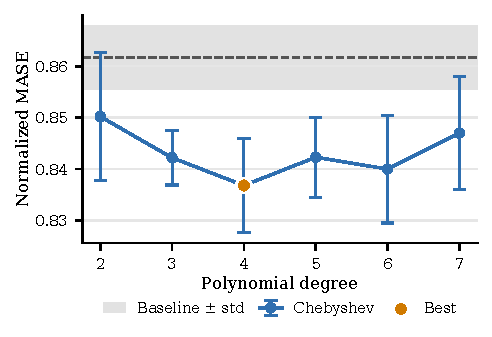
\includegraphics[width=0.66\linewidth]{figures/degree_sweep_line.pdf}
\caption{Chebyshev polynomial degree sweep on GIFT-Eval. Points are 5-seed means with cross-seed standard deviation. The grey band is the baseline mean $\pm$ one standard deviation.}
\label{fig:degree}
\end{figure}

\begin{figure}[H]
\centering
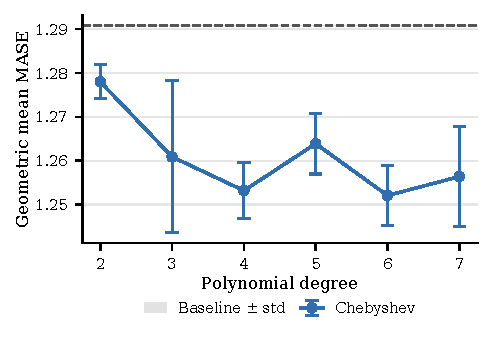
\includegraphics[width=0.66\linewidth]{figures/fev_degsweep.pdf}
\caption{FEV-Bench polynomial degree sweep. Every tested degree improves over the baseline, and the curve is shallow.}
\label{fig:fevdegree}
\end{figure}

The degree sweep tests Chebyshev degrees $2$ through $7$. Every tested degree improves over baseline on both GIFT-Eval and FEV-Bench. Degree 4 is the best mean on GIFT-Eval, while degree 6 is marginally best on FEV-Bench. I therefore treat degree 4 as a strong default rather than a sharply tuned optimum.

\begin{table}[H]
\centering
\caption{Learned coefficients compared with fixed Chebyshev coefficients, seed 0, 10K steps.}
\begin{tabular}{lccc}
\toprule
Setting & Coefficients $(c_1,\ldots,c_4)$ & MASE & $\Delta$\% \\
\midrule
\textbf{Fixed Chebyshev} & $[0,-1,0,0.125]$ & \textbf{0.8234} & \textbf{$-4.99\%$} \\
Learned, Chebyshev init & $[-0.026,-1.032,-0.123,0.007]$ & 0.8332 & $-3.85\%$ \\
Learned, zero init & $[0.308,0.177,0.057,0.045]$ & 0.8358 & $-3.57\%$ \\
\bottomrule
\end{tabular}
\label{tab:learned}
\end{table}

One of the most surprising findings is that the fixed Chebyshev coefficients outperform learned coefficient vectors, even when the learned model is initialized at the Chebyshev coefficients. The learned models still beat baseline, but the fixed polynomial is better. This suggests that the Chebyshev channel acts as an inductive bias rather than just a convenient initialization.

\subsection{Extended Training and Training Dynamics}

\begin{table}[H]
\centering
\caption{100K-step GIFT-Eval results. MASE is normalized geometric mean; standard deviation is cross-seed.}
\begin{tabular}{lccc}
\toprule
Method & MASE & $\Delta$\% vs Baseline & Std \\
\midrule
\textbf{\texttt{d4\_dropout} (ours)} & \textbf{0.8443} & \textbf{$-3.88\%$} & \textbf{0.0079} \\
Baseline & 0.8784 & --- & 0.0189 \\
Duplicate control & 0.8860 & $+0.86\%$ & 0.0083 \\
Zero control & 0.8937 & $+1.73\%$ & 0.0353 \\
\bottomrule
\end{tabular}
\label{tab:100k}
\end{table}

\begin{figure}[H]
\centering
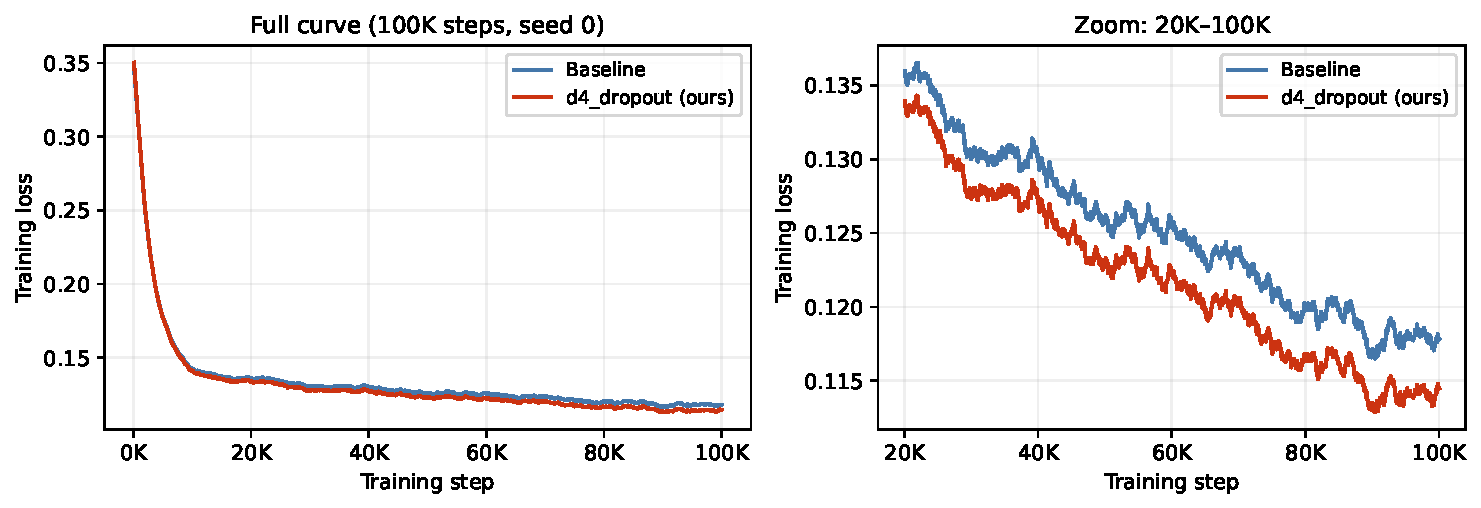
\includegraphics[width=0.86\linewidth]{figures/fig_training_loss_main.pdf}
\caption{Training loss over 100K steps, seed 0, EMA-smoothed. The polynomial model separates early and remains lower throughout training.}
\label{fig:train}
\end{figure}

At 100K steps, the improvement grows from 2.9\% to 3.9\%. The training-loss curves also show that the polynomial model maintains lower loss through the run, especially after the first 20K steps. This is useful evidence that the preconditioning channel continues to help as training proceeds rather than only helping early optimization.

\subsection{Horizon Stratification}

\begin{table}[H]
\centering
\caption{Horizon stratification on GIFT-Eval. Values are 5-seed cross-configuration geometric-mean MASE; percentages are relative to baseline within each bin.}
\begin{tabular}{lcccc}
\toprule
Term & $n$ & Baseline & \texttt{d4} & \texttt{d4\_dropout} \\
\midrule
Short & 55 & 0.840 & \textbf{0.825} ($-1.8\%$) & 0.828 ($-1.4\%$) \\
Medium & 21 & 0.859 & 0.830 ($-3.4\%$) & \textbf{0.823} ($-4.2\%$) \\
Long & 21 & 0.924 & 0.880 ($-4.7\%$) & \textbf{0.874} ($-5.3\%$) \\
\bottomrule
\end{tabular}
\label{tab:horizon}
\end{table}

The improvement is largest on long-horizon tasks. This is consistent with the role of channel dropout: at longer autoregressive horizons, the preconditioning residual increasingly depends on model-generated history rather than fully observed context, so dropout during training makes the model more robust to imperfect or partially synthetic residual information.

\section{Discussion}

This work shows that a small fixed input transformation can improve a modern time-series foundation model. The method is attractive because it is architecture-light: it does not change the transformer stack, the attention mechanism, the output head, or the forecasting target. It simply exposes a theory-guided cross-patch signal before tokenization.

The most important empirical conclusion is that the gain is not an artifact of additional parameters. The Zero and Duplicate controls have the same widened projection as the polynomial model, but they do not reproduce the effect. The fixed Chebyshev channel also beats learned coefficient vectors, which suggests that the polynomial structure itself is doing useful work.

From an ML/statistics perspective, the project combines model design, controlled experimentation, benchmark evaluation, and paired statistical testing. The evaluation spans two benchmarks, multiple seeds, capacity controls, degree sweeps, learned-coefficient ablations, and a longer training budget. Together, these results support the claim that theory-guided input preconditioning is a practical way to improve compact zero-shot forecasters.

\section{Conclusion}

Polynomial input preconditioning adapts Universal Sequence Preconditioning to offline zero-shot time-series forecasting. By concatenating a fixed Chebyshev residual as an auxiliary input channel, it improves Moirai 2.0 Small by 2.9\% on GIFT-Eval and by a similar margin on FEV-Bench while adding only 0.11\% parameters. At 100K training steps, the improvement reaches 3.9\%. These results suggest that foundation models can benefit not only from scale, but also from simple, structured transformations placed before tokenization.

\section*{Acknowledgements and Contributions}

This project was carried out in collaboration with Alex Kawaja, whom I thank for working with me throughout the project. My individual contributions to this CSML independent-work submission were implementing polynomial input preconditioning in the Moirai 2.0 codebase, designing and running the controlled GIFT-Eval and FEV-Bench experiments, conducting the seed analyses and ablations, performing the statistical comparisons, and preparing the paper, poster, and presentation materials. Alex contributed through joint project discussion, experimental planning, debugging and evaluation support, and interpretation of results.

\bibliographystyle{plainnat}
\bibliography{references}

\end{document}
